\documentclass[11pt, a4paper]{article}
\usepackage{pdfpages}
\usepackage{parallel}
\usepackage[T2A]{fontenc}
\usepackage{ucs}
\usepackage[utf8x]{inputenc}
\usepackage[polish,english,russian]{babel}
\usepackage{hyperref}
\usepackage{rotating}
\usepackage[inner=2cm,top=1.8cm,outer=2cm,bottom=2.3cm,nohead]{geometry}
\usepackage{listings}
\usepackage{graphicx}
\usepackage{wrapfig}
\usepackage{longtable}
\usepackage{indentfirst}
\usepackage{array}
\usepackage{tikzsymbols}
\usepackage{soul}
\usepackage[ruled,vlined]{algorithm2e}
%\counterwithout{figure}{section} 

\usepackage{url}
\makeatletter
\g@addto@macro{\UrlBreaks}{\UrlOrds}
\makeatother

\newcolumntype{P}[1]{>{\raggedright\arraybackslash}p{#1}}
\frenchspacing
\usepackage{fixltx2e} %text sub- and superscripts
\usepackage{icomma} % коскі ў матэматычным рэжыме
\PreloadUnicodePage{4}

\newcommand{\longpage}{\enlargethispage{\baselineskip}}
\newcommand{\shortpage}{\enlargethispage{-\baselineskip}}

\def\switchlang#1{\expandafter\csname switchlang#1\endcsname}
\def\switchlangbe{
\let\saverefname=\refname%
\def\refname{Літаратура}%
\def\figurename{Іл.}%
}
\def\switchlangen{
\let\saverefname=\refname%
\def\refname{References}%
\def\figurename{Fig.}%
}
\def\switchlangru{
\let\saverefname=\refname%
\let\savefigurename=\figurename%
\def\refname{Литература}%
\def\figurename{Рис.}%
}

\hyphenation{admi-ni-stra-tive}
\hyphenation{ex-pe-ri-ence}
\hyphenation{fle-xi-bi-li-ty}
\hyphenation{Py-thon}
\hyphenation{ma-the-ma-ti-cal}
\hyphenation{re-ported}
\hyphenation{imp-le-menta-tions}
\hyphenation{pro-vides}
\hyphenation{en-gi-neering}
\hyphenation{com-pa-ti-bi-li-ty}
\hyphenation{im-pos-sible}
\hyphenation{desk-top}
\hyphenation{elec-tro-nic}
\hyphenation{com-pa-ny}
\hyphenation{de-ve-lop-ment}
\hyphenation{de-ve-loping}
\hyphenation{de-ve-lop}
\hyphenation{da-ta-ba-se}
\hyphenation{plat-forms}
\hyphenation{or-ga-ni-za-tion}
\hyphenation{pro-gramming}
\hyphenation{in-stru-ments}
\hyphenation{Li-nux}
\hyphenation{sour-ce}
\hyphenation{en-vi-ron-ment}
\hyphenation{Te-le-pathy}
\hyphenation{Li-nux-ov-ka}
\hyphenation{Open-BSD}
\hyphenation{Free-BSD}
\hyphenation{men-ti-on-ed}
\hyphenation{app-li-ca-tion}

\def\progref!#1!{\texttt{#1}}
\renewcommand{\arraystretch}{2} %Іначай формулы ў матрыцы зліпаюцца з лініямі
\usepackage{array}

\def\interview #1 (#2), #3, #4, #5\par{

\section[#1, #3, #4]{#1 -- #3, #4}
\def\qname{LVEE}
\def\aname{#1}
\def\q ##1\par{{\noindent \bf \qname: ##1 }\par}
\def\a{{\noindent \bf \aname: } \def\qname{L}\def\aname{#2}}
}

\def\interview* #1 (#2), #3, #4, #5\par{

\section*{#1\\{\small\rm #3, #4. #5}}
\ifx\ParallelWhichBox\undefined%
    \addcontentsline{toc}{section}{#1, #3, #4}%
\else%
\ifnum\ParallelWhichBox=0%
    \addcontentsline{toc}{section}{#1, #3, #4}%
\fi\fi%

\def\qname{LVEE}
\def\aname{#1}
\def\q ##1\par{{\noindent \bf \qname: ##1 }\par}
\def\a{{\noindent \bf \aname: } \def\qname{L}\def\aname{#2}}
}

\newcommand{\interviewfooter}[1]{
\vskip 1em
\noindent \textit{#1}
}


\begin{document}

\title{1993 "--- Prohance mouse}
\date{}
\maketitle

Манипулятор Prohance, выпущенный в 1993, ориентирован в первую очередь на пользователей электронных таблиц Lotus 1-2-3, которые не хотят постоянно перемещать руку с мыши на клавиатуру и обратно. Чтобы решить их проблему, 
    Prohance mouse содержит в переденй части корпуса дополнительную функциональную клавиатуру.
    
    \begin{figure}[h]
        \centering
    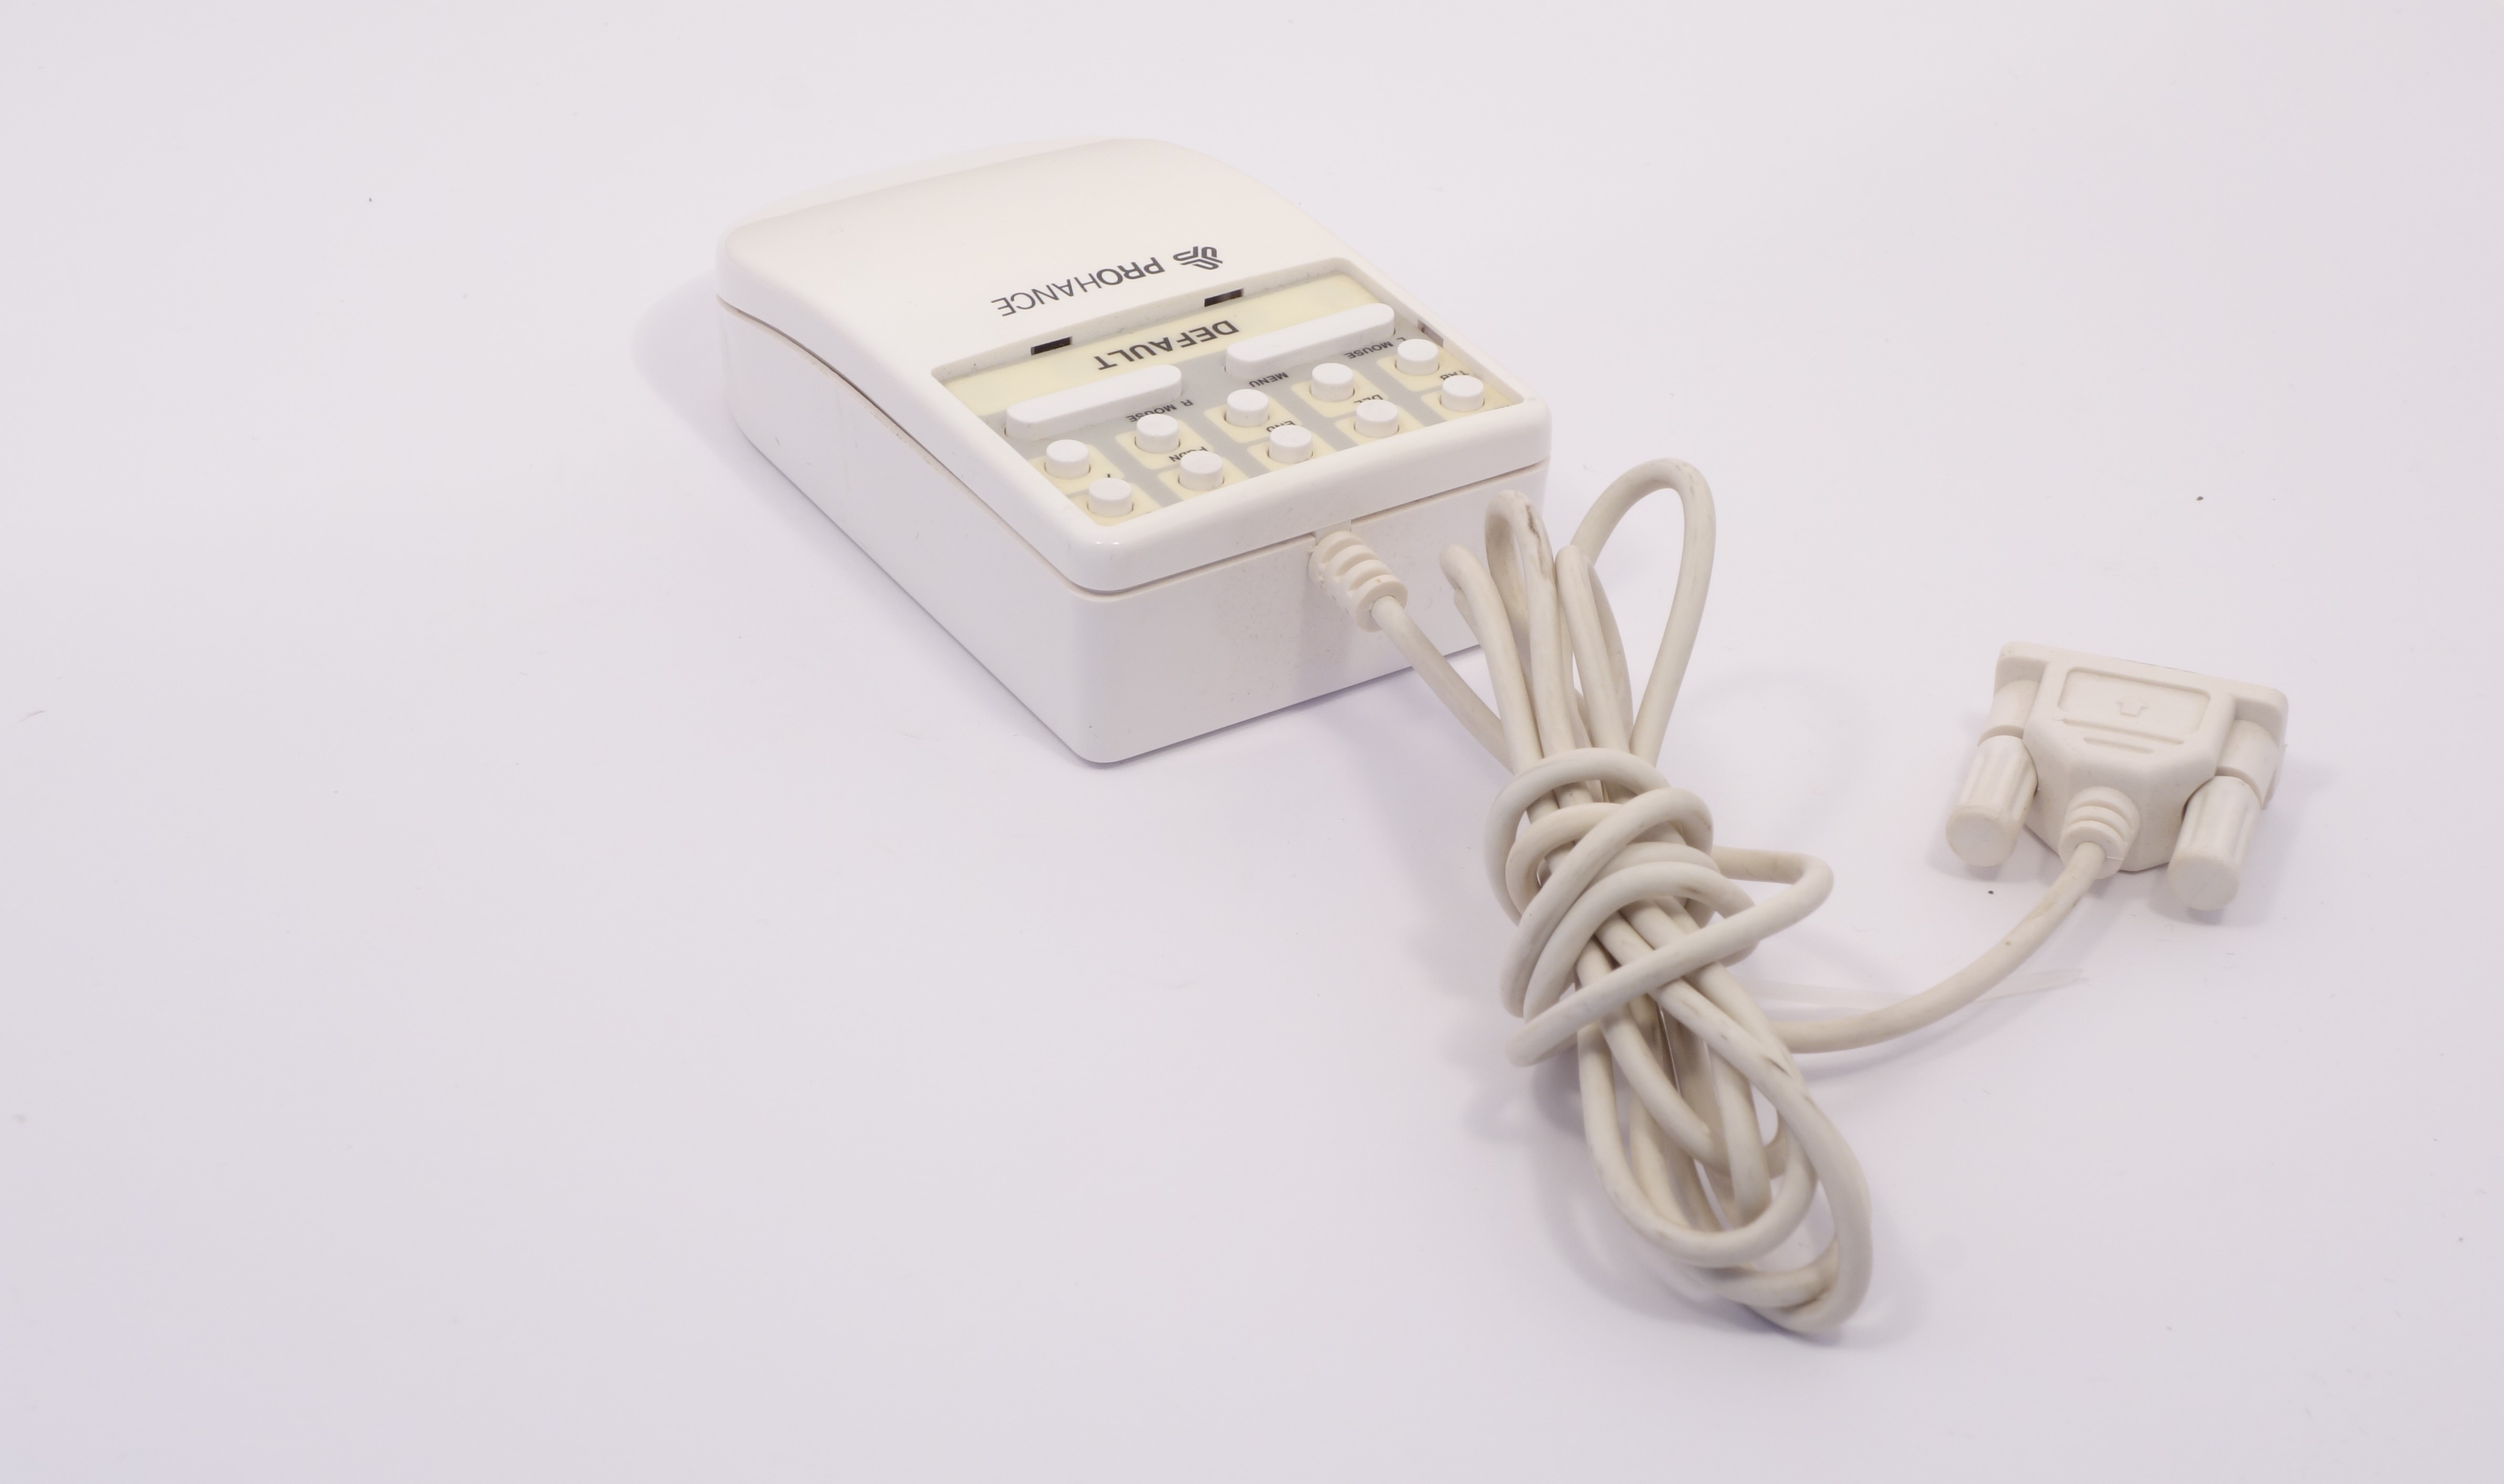
\includegraphics[scale=0.4]{5.1jpg.jpg}
        \label{quad-niz}
        \caption{Изображение Prohance mouse}
    \end{figure}
    
    При работе с Lotus 1-2-3, для которого она специально разработана, данная мышь покаызвает себя достаточно эффективно. В других приложениях и графических оболочках (например, PC Paintbrush и GEM) она действует как любая другая мышь. Однако в ранней версии драйвера содержались ошибки, приводившие к тому что даже незначительное перемещение мыши в Microsoft Word приводило к пролистыванию страниц (в обновленном драйвере было исправлено несколько ошибок, включая эту). Что касается кнопок Prohance, в других программах они работали хаотично, либо совсем не работали.
    
    Prohance одинаково работает на коврике для мыши и на деревянной поверхности. Можно установить уровни чувствительности через конфигурационные файлы драйвера.
    
    Prohance показывал достаточно большое ускорение в большинстве приложений; однако драйвер не позволяет регулировать ускорение динамически.
    
    В плане эргономики манипулятор повторяет форму мыши Microsoft, известной как <<Dove Bar mouse>>, позаимствовавшей форму корпуса у шлифовального бруска и потому оказавшейся одной из первых эргономичных мышшей. Поэтому с точки зрения формы к Prohance нет претензий по части эргономики. Однако как основные кнопки, так и дополнительные клавиши Prohance очень мелкие, что весьма невыгодно отличается от продукта Microsoft. К тому же они резиновые на ощупь и издают едва слышный клик при нажатии. При этом они  выдерживают легкое нажатие, поэтому вероятность случайного нажатия на клавиши мала.
    \begin{figure}[h]
        \centering
    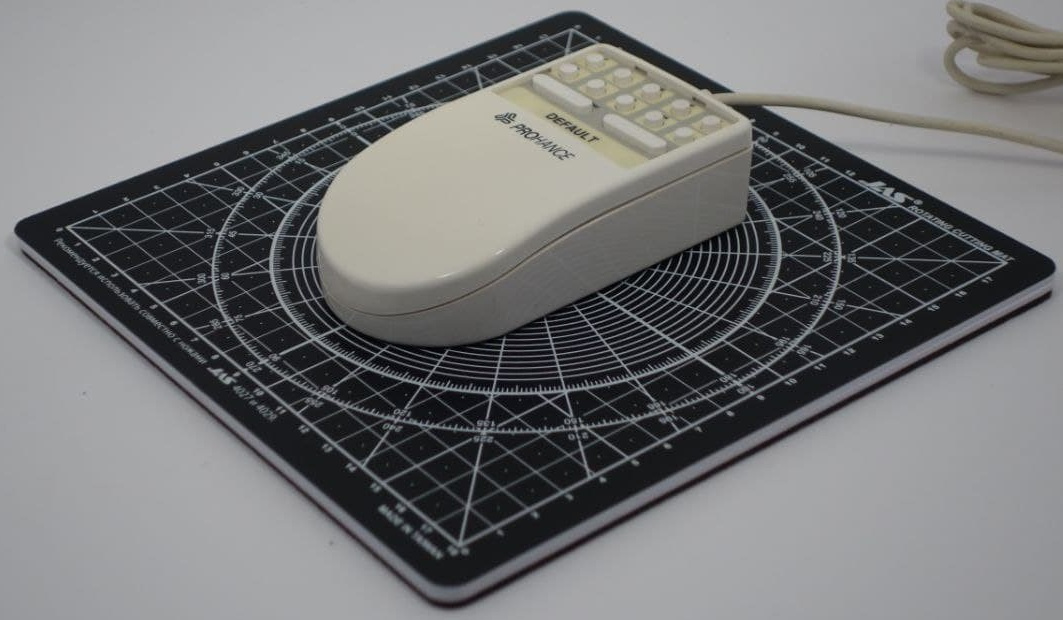
\includegraphics[scale=0.3]{5.3.jpg}
        \label{quad-kov}
        \caption{Изображение Prohance Mouse на размерном коврике с шагом сетки 1~см}
    \end{figure}
    
    
    \begin{figure}[h]
        \centering
    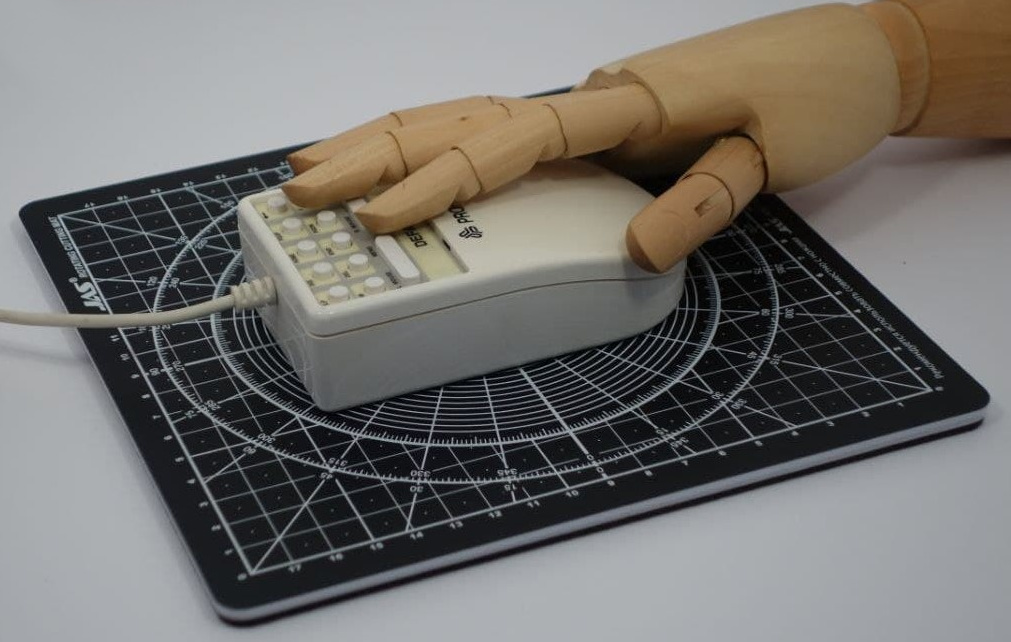
\includegraphics[scale=0.3]{5.2.jpg}
        \label{quad-kov}
        \caption{Изображение Prohance Mouse с моделью руки человека}
    \end{figure}
    
    У мыши нет отличительного признака, который помог бы идентифицировать кнопки мыши. Это особенно актуально для набора дополнительных функциональных клавиш в верхней части мыши. Эти круглые функциональные клавиши одинакового размера, и перед нажатием приходилось постоянно следить за правильным положением пальцев. Производитель предусмотрел возможность сменных вставок - накладок, размещаемых поверх функциональной клавиатуры. Однако из-за размера мыши эти надписи достаточно мелкие, перекрываются пальцами, и нетренированному пользователю приходится пристально их рассматривать, чтобы найти нужную клавишу.
    
    В итоке Prohance Mouse получила плохие оценки пользователей из-за особенностей функциональных клавиш  кнопок.
    
    В отличие от других мышей, драйвер Prohance не имеет экранных меню. Вместо этого он использует переназначение функциональных клавиш. Разработанный в первую очередь для работы с электронными таблицами, он функционирует как дополнительная клавиатура для ввода данных, установленная на мыши.
    
    В консольных приложениях перемещение Prohance воздействует на мигающий текстовый курсор, а не  отдельный курсор мыши. Это означает, что нельзя перемещать мышь в любом месте экрана в текстовом процессоре (только там, где есть текст), а такие приложения, как Lotus, будут издавать звуковой сигнал при перемещаении мыши за пределы диапазона ячеек. Функции, ориентированные на диапазон ячеек, такие как копирование, стирание, перемещение и суммирование, очень полезны, поскольку нужно просто нажать соответствующую кнопку и переместить курсор в желаемый диапазон. Это избавляет от утомительной работы. 
    
    К сожалению, Prohance автоматизирует только несколько функций, которые иногда приходятся кстати, но которых недостаточно, чтобы не переключаться с клавиатуры на мышь и обратно. Однако пользователи, работающие исключительно с табличным процессором Lotus, можгли бы найти эти компромиссы стоящими.
    
    Prohance имеет функцию записи макросов, которая позволяет определять новые шаблоны функциональной клавиатуры мыши для неподдерживаемых приложений, а также изменять существующие шаблоны.
    
    
    Также необходимо заметить, что Prohance Mouse несовместима с Microsoft Mouse. При использовании драйвера Microsoft, мышь Prohance не распознаетcz. Производительность мыши с программным обеспечением, настроенным для драйвера Microsoft, была неоднозначной - некоторые приложения работали, другие - нет, даже при загруженном соответствующем драйвере Prohance для конкретного приложения.

    При этом настроить Prohance достаточно просто. Программа установки автоматизирует шаги, хотя часть, которая устанавливает шаблон клавиатуры по умолчанию, создает впечатление, будто возможно установить несколько шаблонов, хотя на самом деле она установит только один (первый выбранный), который будет инициализирован при запуске. Инструкции по установке в интерактивном режиме должна была бы четко указывать, что пользователь устанавливает шаблон загрузки, и что все остальные автоматически копируются на жесткий диск для использования при необходимости.

   Мышь в разобранном виде показана на рисунке 2.12. Как можно видеть, она представляет собой типичную для 90-х годов оптомеханическую конструкцию, а блок кнопок и функциональных клавиш выполнен на отдельной печатной плате и является миниатюрной мембранной клавиатурой, аналогичной устанавливаемым в карманных микрокалькуляторах.
   
  \begin{figure}[h]
        \centering
    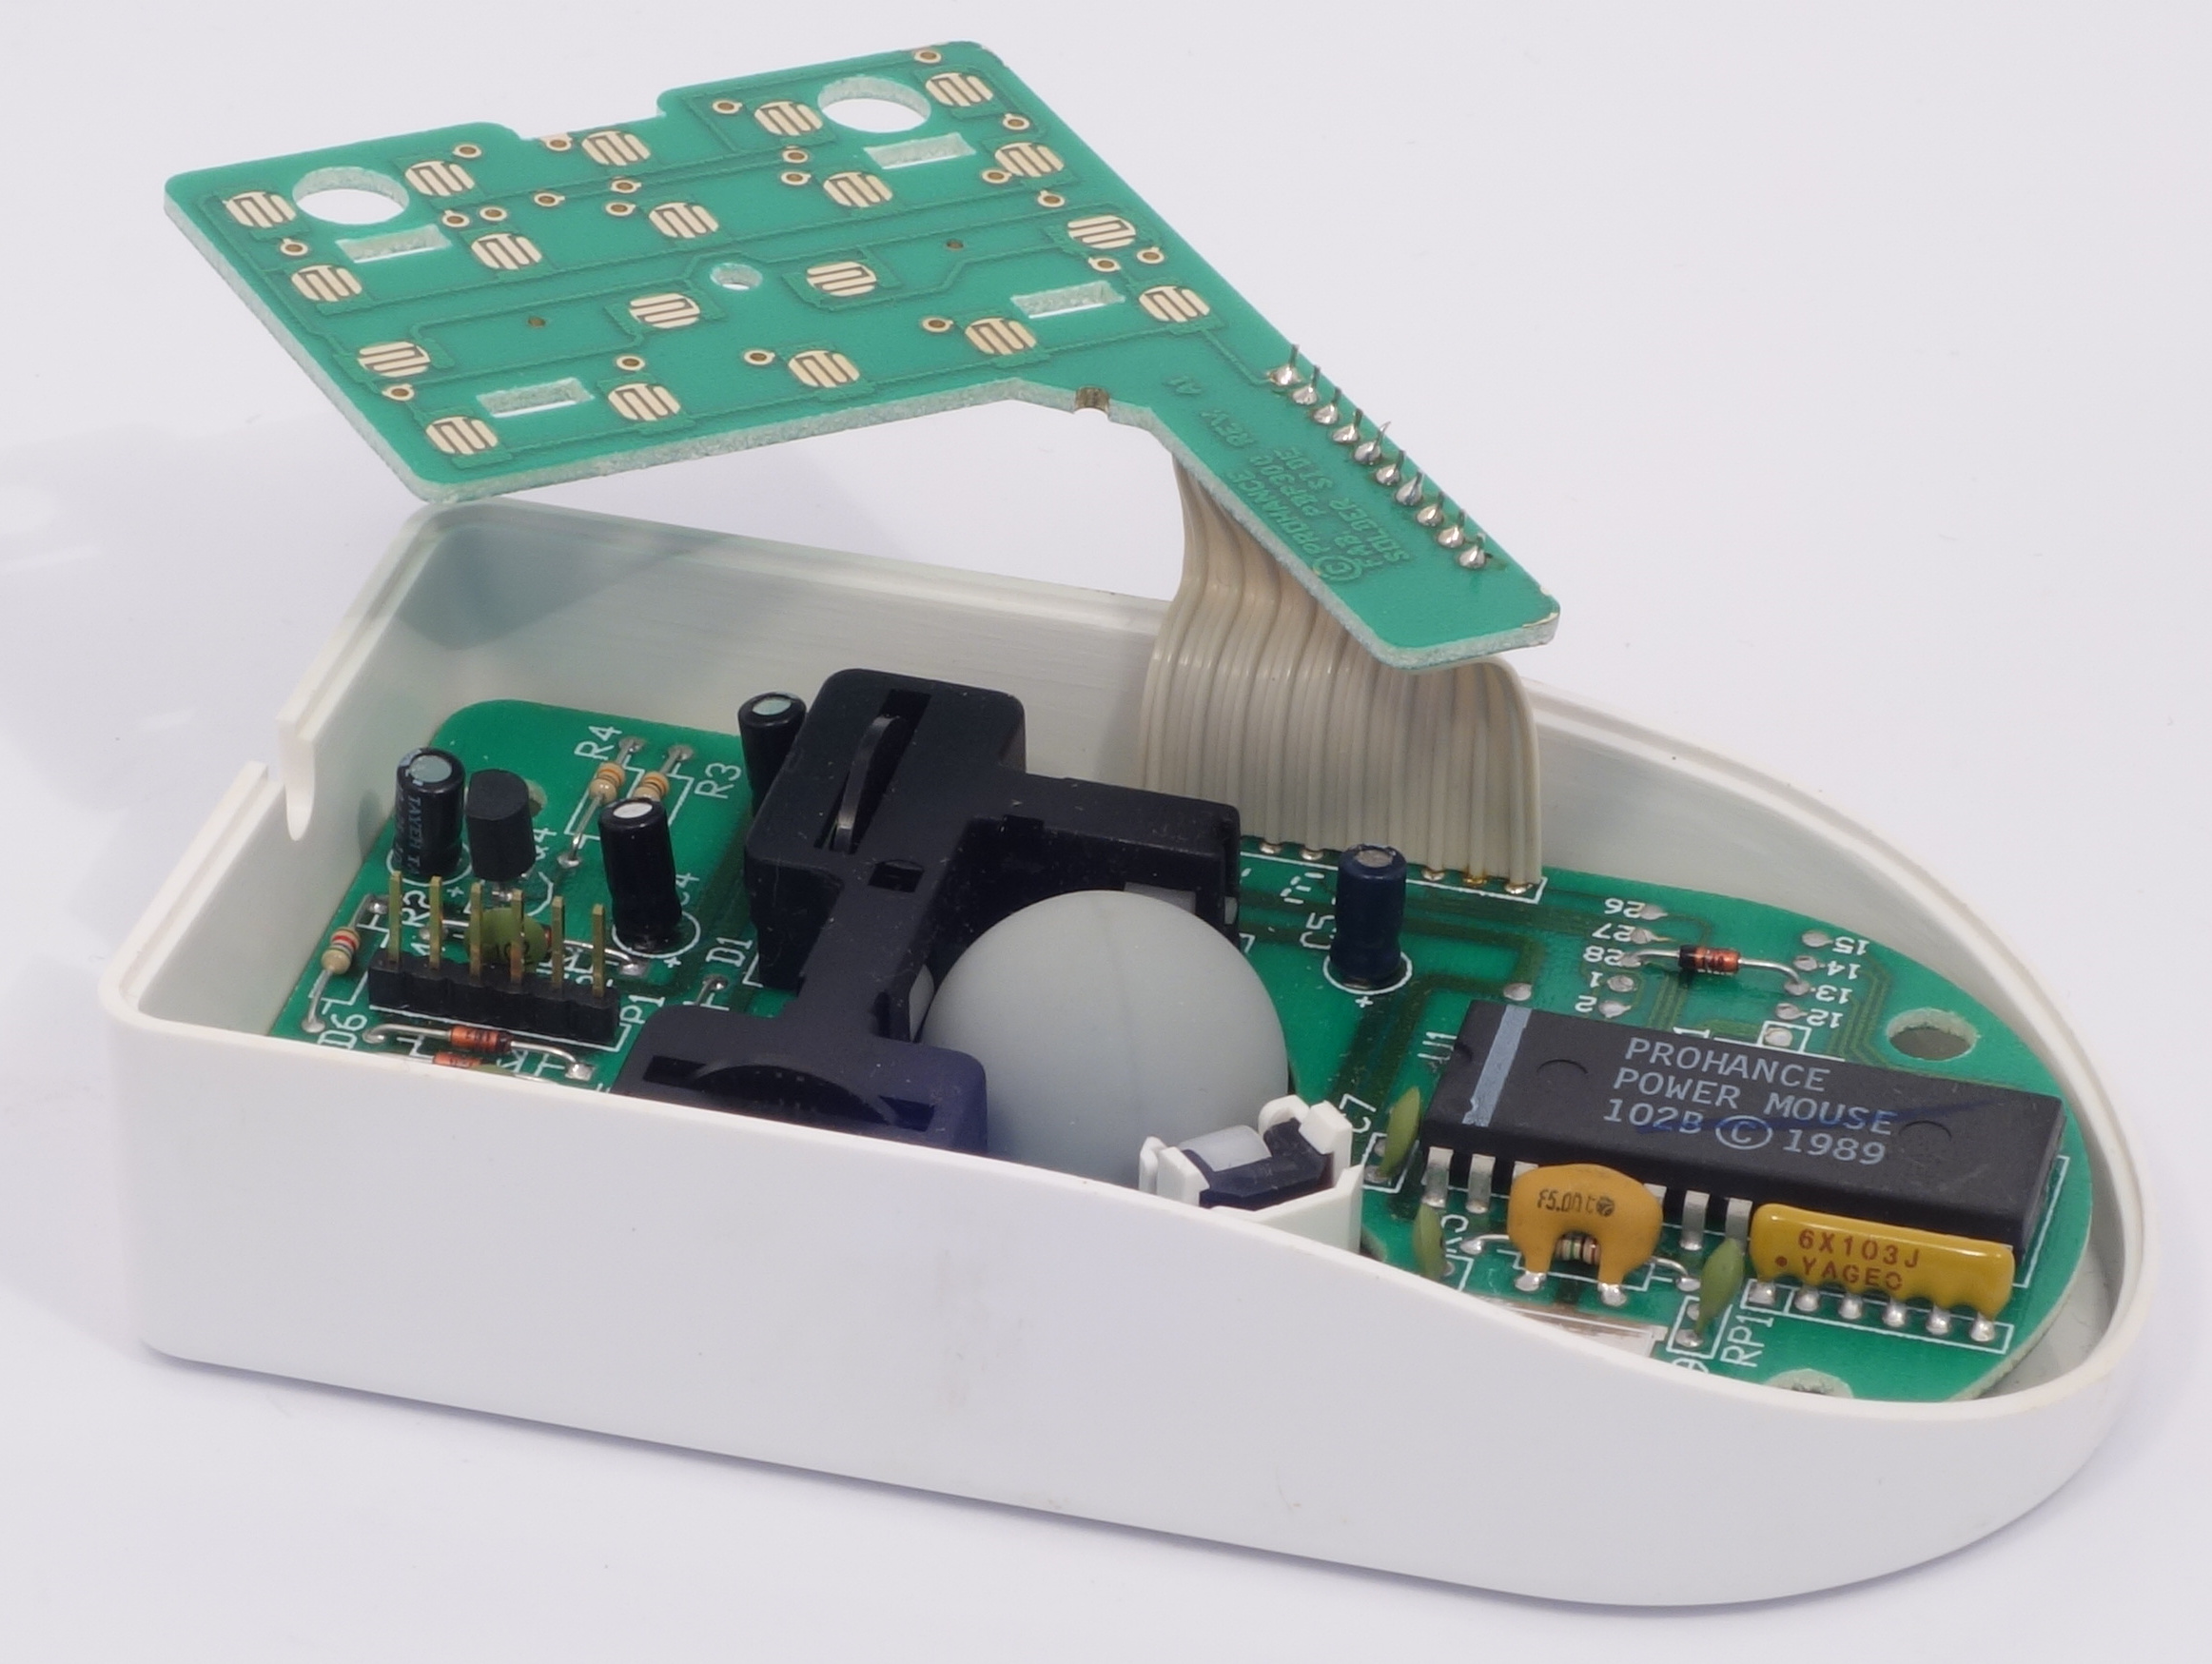
\includegraphics[scale=0.35]{6.1.jpg}
        \label{quad-niz}
        \caption{Изображение Prohance в разобранном виде}
    \end{figure}
\begin{thebibliography}{9}
\bibitem{prohance} Gruman G. What price mice? // Infoworld, V. 12, No. 17, April 23, 1990. - P. 63-69.
\bibitem{livingston} Livingston B. Genetically engineered mice run amok at Windows World // InfoWorld, Vol. 15, Iss. 21, May 24, 1993. - p. 34. https://books.google.by/books?id=PTsEAAAAMBAJ&lpg=PA34&dq=prohance%20mouse&hl=ru&pg=PA34#v=onepage&q=prohance%20mouse&f=false
\end{thebibliography}
\end{document}
